統計情報提供機能は,教材提供者が作成した問題を学習者が解いた際の回答情報を基に,グラフで統計情報を提供する機能である.
これにより,教材提供者は作成したコンテンツの質を向上させることができる.
提示する統計情報の内容としては,問題の各選択肢における割合や回答者の年齢層,性別である.
統計情報提供機能のGUIは図\ref{toukei}の通りである.

\begin{figure}[htbp]
    \begin{center}
        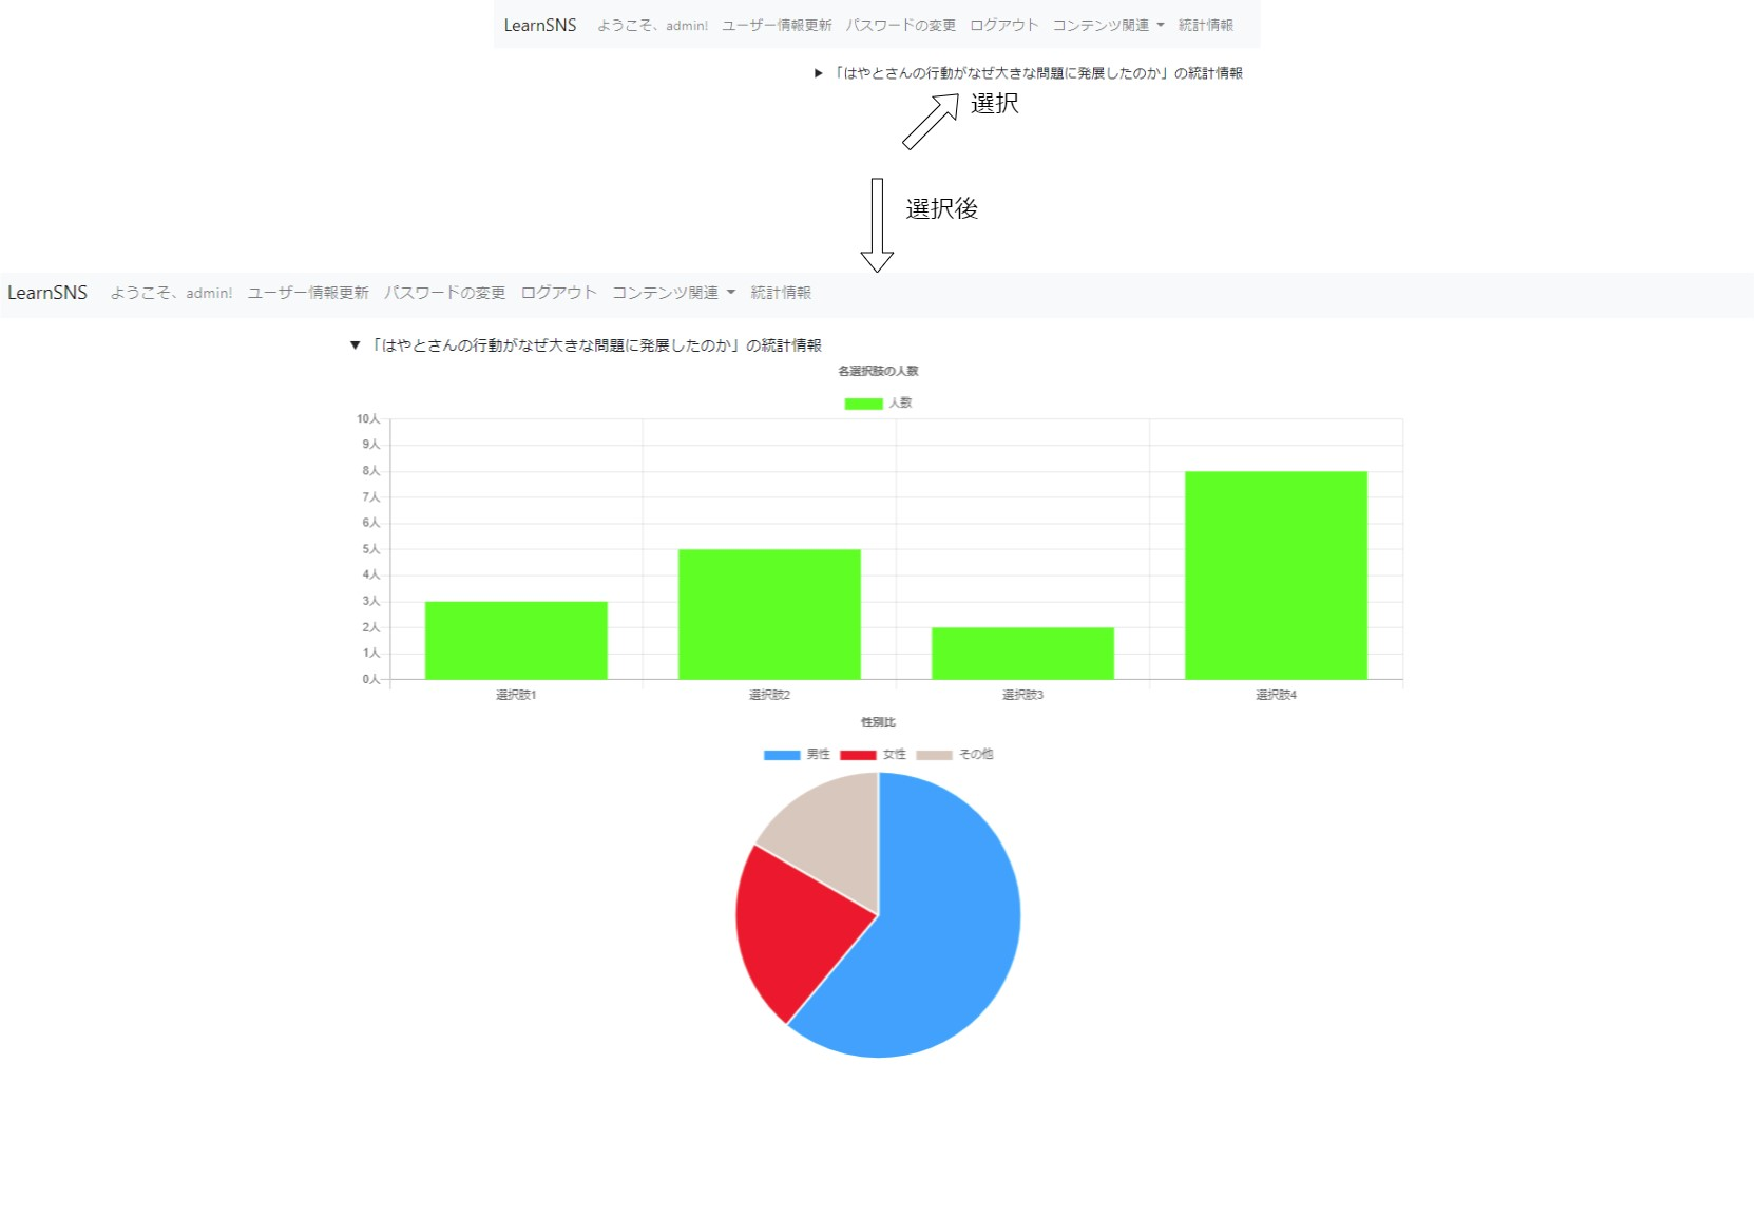
\includegraphics[width=15cm,height=14cm,keepaspectratio]{toukei_ex-crop.pdf}\\
        %includegraphicsの詳しい使い方ははLaTeXの参考書を参照.
    \end{center}
    \caption{統計情報提供機能のGUI}
    \label{toukei}
\end{figure}

\newpage
本機能はChart.jsというjavascriptで作成されたグラフ描画ライブラリを作成している.
Chart.jsでは線グラフ,棒グラフ,レーダーチャート,鶏頭図,ドーナツチャート,円グラフ,バブルチャートを作成できる.
本機能では,棒グラフと円グラフを使用している.

また,本機能で取得可能な情報を表\ref{info}に示す.
これらの取得できる情報を使って教材提供者はChart.jsで新たなグラフを挿入することができる.

\begin{table}[htb]
    \begin{center}
        \caption{取得可能情報一覧}
            \begin{tabular}{|l|l|} \hline
                取得可能情報 & 詳細 \\ \hline
                学習者情報 &   
                \begin{tabular}{l}
                    年齢\\性別\\回答した問題・選択肢 
                \end{tabular}\\ \hline
                コンテンツ情報 & 問題に対応したコンテンツ \\ \hline
            \end{tabular}
    \label{info}
    \end{center}
\end{table}